% File SDSS2020_SampleExtendedAbstract.tex
\documentclass[10pt]{article}
\usepackage{sdss2020} % Uses Times Roman font (either newtx or times package)
\usepackage{url}
\usepackage{latexsym}
\usepackage{amsmath, amsthm, amsfonts}
\usepackage{algorithm, algorithmic}
\usepackage{graphicx}
\usepackage{adjustbox}
\graphicspath{{images/}}

\title{Artificial Neural Networks and Deep Learning \\
Homework 1}

\author{
  Nicola Dean \\
  10617541 \\
  {\tt nicola.dean \\
  \tt @mail.polimi.it} \\\And
  Marco Fasanella \\
  10617541 \\
  {\tt marco.fasanella \\
  \tt @mail.polimi.it} \\\And
  Raffaello Fornasiere \\
    10617541 \\
    {\tt raffaello.fornasiere \\
    \tt @mail.polimi.it} \\\And
  Christian Spano \\
  10617541 \\
  {\tt christian.spano \\
  \tt @mail.polimi.it} \\}


\date{}

\begin{document}
\maketitle
%\begin{abstract}

%\end{abstract}

%{\bf Keywords:} VGG16, VGG19, Helpful

\section{Introduction}
In order to touch all the important aspects of the procedure of finding the best solution to this classification problem,
we started from our own self-made model to more sophisticated methodologies.\\
 We can summarize our approaches in:
\begin{itemize}
  \item Vanilla network
  \item Transfer Learning and Fine Tuning
  \item Ensemble method
\end{itemize}
Furthermore in all the attempts made, we used two classes, specifically \textbf{created to automate and support the model creation
procedure}:
\begin{itemize}
  \item Dataset Helper
  \item Model Helper
\end{itemize}
Through the continuous attempts, and support of methods in the two helper classes, we managed to find our best model and
reach 0.8691 accuracy in the competiton.


\section{Dataset Helper and Model Helper}
--CHRISTIAN--
Spiegazione delle due classi: \
lista delle funzioni e automatizzazione

\section{First try: vanilla network}
--NICOLA--
-IMG della rete (dal lab) (magari orizzontale)
risultati
considerazioni
\subsection{Batch Normalization}
A first attempt was also adding a Batch Normalization + Relu Activation Layer before our Pooling layers.\
This lead to poor result due to the fact that the network was too small.
\subsection{Our homemade CNN}
So deepening the CNN gave this solution much significant improvements.\\
METTERE IMMAGINE CNN FINALE
--- RAFFAELLO---


\subsection{Considerations}
Best result consideration and observations
\section{Transfer Learning and Fine Tuning}
We then noticed that we needed a big change on the approach to use, because the homemade
CNN was performant, but not enough. So \textbf{we started using transfer learning and Fine tuning}

\subsection{Approach: Freezing Layers}
The \textit{modus operandi} that will be used from now is: freezing all layers while training on our augmented dataset the keras.application
CNN, and then unlock a small amount of layers to the second phase of training (fine tuning) as near as possible to the output.
\subsection{VGG19}
VGG-19 is a convolutional neural network that is 19 layers deep, so we kept the freezed layers in the range of the first 8-14.\\
Different Data Augmentations (with different seeds and augmentation parameters) were performed between the two phases,
to even increase randomisation in the two training processes.
\subsubsection{Results}
\begin{table}[ht]
\centering
\begin{adjustbox}{width=240}
\small
\begin{tabular}{|c|l|l|l|l|l}

\hline \bf Freezed Layers & \bf Accuracy & \bf Precision & \bf Recall & \bf F1 \\ \hline
8 & 0.8169 & 0.7989 & 0.7651 & 0.763\\
9 & 0.8225 & 0.8181 & 0.7682 & 0.7776\\
10 & 0.8338 & 0.8161 & 0.7929 & 0.8001\\
11 & 0.7577 & 0.7109 & 0.715 & 0.7048\\
12 & 0.7944 & 0.766 & 0.7504 & 0.7489\\
13 & 0.8028 & 0.7806 & 0.754 & 0.7596\\
\hline
\end{tabular}
\end{adjustbox}
\caption{Results with Transfer Learning and Number of freezed layers for VGG19.}
\end{table}


\begin{figure}[ht]
\begin{center}
\centerline{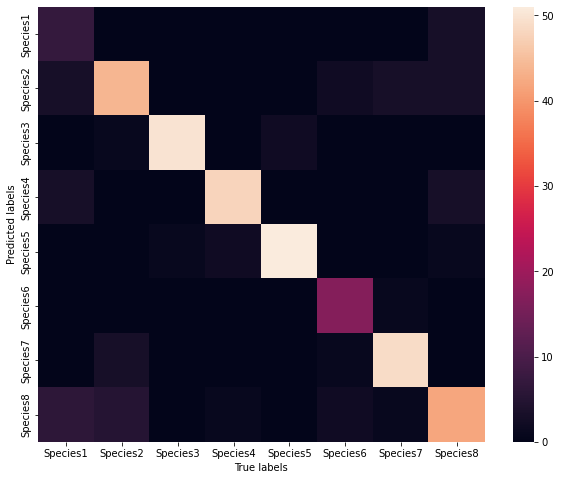
\includegraphics[width=\columnwidth]{VGG19_best}}
\caption{Confusion Matrix of best configuration with VGG19.}
\label{bayespic}
\end{center}
\end{figure}
\subsubsection{Considerations}
One of the most particular observation that we can made after experimenting the first attempts of freezing, is that freezing the net
until the pooling and not between convolutions leads to a better accuracy.

\subsection{VGG16}
--CHRISTIAN--
Spiegazione modell + prove fatte
\subsubsection{Results}
\subsection{Xception}

\subsection{Other Models}
\subsubsection{Resnet}
--NICOLA--
\subsubsection{GoogleNet}
\subsection{EfficientNet}
--NICOLA--



\section{Ensemble}
--NICOLA--
Approccio
provato a mischiare modelli
          c'era bias perchè avevano seed diversi
\subsubsection{Results}



\section{If we had more time..}
con più tempo cosa avremmo provato




\section{Our Submissions}
\begin{table}[ht]
\centering
\begin{adjustbox}{width=240}
\small
\begin{tabular}{|c|l|l|l|l|l}

\hline \bf Description & \bf Result \\ \hline
VGG19 - 10 Freezed Layers & 0.823015873 \\
b & 0.8225 \\

\hline
\end{tabular}
\end{adjustbox}
\caption{Results with Transfer Learning and Number of freezed layers for VGG19.}
\end{table}
%{\bf Footnotes}: Note di sotto.}.
\section{Conclusions}
Considerazioni finali e best model fattoo
\bibliographystyle{sdss2020} % Please do not change the bibliography style
\bibliography{SampleReferencesForExtendedAbstract}

\end{document}
